\documentclass[11pt,a4paper]{article}
\usepackage[utf8]{inputenc}
\usepackage[T1]{fontenc}
\usepackage{amsmath,amssymb,amsfonts}
\usepackage{graphicx}
\usepackage{booktabs}
\usepackage{hyperref}
\usepackage{geometry}
\usepackage{listings}
\usepackage{xcolor}
\usepackage{caption}
\usepackage{float}
\usepackage{enumitem}
\usepackage{tikz}
\usepackage{longtable}
\usepackage{algorithm}
\usepackage{algorithmic}
\usepackage{mdframed}

\geometry{margin=2.5cm}

\definecolor{codegreen}{rgb}{0,0.6,0}
\definecolor{codegray}{rgb}{0.5,0.5,0.5}
\definecolor{codepurple}{rgb}{0.58,0,0.82}
\definecolor{backcolour}{rgb}{0.95,0.95,0.92}
\definecolor{warningcolor}{rgb}{1.0,0.95,0.8}
\definecolor{infocolor}{rgb}{0.9,0.95,1.0}

\lstdefinestyle{mystyle}{
    backgroundcolor=\color{backcolour},   
    commentstyle=\color{codegreen},
    keywordstyle=\color{magenta},
    numberstyle=\tiny\color{codegray},
    stringstyle=\color{codepurple},
    basicstyle=\ttfamily\footnotesize,
    breakatwhitespace=false,         
    breaklines=true,                 
    captionpos=b,                    
    keepspaces=true,                 
    numbers=left,                    
    numbersep=5pt,                  
    showspaces=false,                
    showstringspaces=false,
    showtabs=false,                  
    tabsize=2
}

\lstset{style=mystyle}

\title{\textbf{AADS-ULoRA v5.5 Mobile Integration Guide}\\Cloud-Based Inference Architecture for\\Uyumsoft ZiraiTakip Mobile Application}
\author{Agricultural AI Development Team\\Industrial Engineering Graduation Project}
\date{March 2026--Version 5.5}

\begin{document}

\maketitle

\begin{abstract}
This document specifies the complete mobile integration architecture for AADS-ULoRA v5.5 within the existing Uyumsoft ZiraiTakip mobile application. The system employs a cloud-based inference model where DINOv3-powered crop adapters run on GPU servers, while the mobile application handles image capture, preprocessing, offline queueing, and result presentation. Key features include: (1) RESTful API contract between mobile and cloud; (2) intelligent offline queueing with automatic synchronization; (3) real-time OOD notifications for novel disease detection; (4) background adapter updates; and (5) bandwidth-efficient image transmission. This architecture enables farmers to diagnose plant diseases in real-time while allowing the system to continuously learn from field data without interrupting user experience.
\end{abstract}

\tableofcontents
\newpage

\section{Executive Summary}

\subsection{Deployment Architecture}

\begin{figure}[H]
\centering
\begin{tikzpicture}[scale=0.8, transform shape,
    box/.style={rectangle, draw, rounded corners, minimum width=3cm, minimum height=1cm, align=center},
    cloud/.style={ellipse, draw, minimum width=3cm, minimum height=1.5cm, align=center, fill=gray!10},
    arrow/.style={->, >=stealth, thick}]
    
    % Mobile side
    \node[box, fill=blue!10] (camera) at (0,0) {Camera\\Module};
    \node[box, fill=blue!10] (preprocess) at (0,-2) {Image\\Preprocessing};
    \node[box, fill=blue!10] (queue) at (0,-4) {Offline\\Queue};
    \node[box, fill=blue!10] (ui) at (0,-6) {Results\\UI};
    
    % Cloud side
    \node[cloud] (router) at (6,0) {Crop Router\\(DINOv3-base)};
    \node[cloud] (adapter) at (6,-2.5) {Crop Adapter\\(DINOv3-giant)};
    \node[cloud] (ood) at (6,-5) {OOD Detector\\(Dynamic Mahalanobis)};
    
    % Backend
    \node[box, fill=green!10] (db) at (10,-2.5) {Adapter\\Registry};
    \node[box, fill=green!10] (storage) at (10,-5) {Sample\\Storage};
    
    % Connections
    \draw[arrow] (camera) -- (preprocess);
    \draw[arrow] (preprocess) -- node[left] {HTTP/2} node[right] {(online)} (queue);
    \draw[arrow] (queue) -- node[above] {Base64 JPEG} (router);
    \draw[arrow] (router) -- (adapter);
    \draw[arrow] (adapter) -- (ood);
    \draw[arrow] (ood) -- (ui);
    \draw[arrow] (adapter) -- (db);
    \draw[arrow] (ood) -- (storage);
    
    % Feedback loop
    \draw[arrow, dashed] (storage) -- node[below] {Phase 2/3} node[above] {trigger} (adapter);
    
\end{tikzpicture}
\caption{Cloud-Based Mobile Integration Architecture}
\end{figure}

\subsection{Key Design Decisions}

\begin{mdframed}[backgroundcolor=infocolor, roundcorner=5pt]
\begin{enumerate}[leftmargin=*]
    \item \textbf{Cloud Inference:} DINOv3-giant (1.1B parameters) runs on GPU servers; mobile only handles UI and networking
    \item \textbf{Offline-First:} Queue-based architecture ensures functionality in poor connectivity areas
    \item \textbf{Incremental Updates:} Adapters update via background download; no app store release needed
    \item \textbf{OOD Feedback Loop:} Novel detections trigger expert labeling, enabling continuous learning
\end{enumerate}
\end{mdframed}

\section{System Architecture}

\subsection{Mobile Application Components}

\begin{table}[H]
\centering
\caption{Mobile Component Responsibilities}
\begin{tabular}{lp{4cm}p{6cm}}
\toprule
\textbf{Component} & \textbf{Technology} & \textbf{Responsibilities} \\
\midrule
Image Capture & CameraX (Android) / AVFoundation (iOS) & Capture, focus, exposure, flash control \\
Preprocessing & OpenCV Mobile / Core Image & Resize to 224$\times$224, normalize, quality check \\
Network Layer & OkHttp / Alamofire & HTTP/2, retry logic, certificate pinning \\
Offline Queue & Room (Android) / Core Data (iOS) & SQLite persistence, sync scheduling \\
Results UI & Jetpack Compose / SwiftUI & Confidence visualization, OOD warnings, history \\
Push Handler & Firebase Cloud Messaging & Adapter updates, Phase 2/3 completion alerts \\
\bottomrule
\end{tabular}
\end{table}

\subsection{Cloud Infrastructure Components}

\begin{table}[H]
\centering
\caption{Cloud Component Specifications}
\begin{tabular}{lp{4cm}p{6cm}}
\toprule
\textbf{Component} & \textbf{Technology} & \textbf{Specifications} \\
\midrule
API Gateway & NGINX / AWS ALB & SSL termination, rate limiting, request routing \\
Crop Router Service & FastAPI + DINOv3-base & 86M params, 50ms inference, CPU/GPU flexible \\
Adapter Service & FastAPI + DINOv3-giant & 1.1B params, 200ms inference, GPU required (A100) \\
OOD Detector & Dynamic Mahalanobis & Per-class thresholds, 10ms overhead \\
Adapter Registry & PostgreSQL + Redis & Metadata, OOD statistics, caching \\
Sample Storage & AWS S3 / MinIO & Raw images, OOD candidates, training batches \\
Training Pipeline & PyTorch + PEFT & Async Phase 2/3 training, model versioning \\
\bottomrule
\end{tabular}
\end{table}

\section{API Contract}

\subsection{Base Configuration}

\begin{mdframed}[backgroundcolor=backcolour, roundcorner=5pt]
\begin{lstlisting}[language=bash]
# Base URL (configurable per deployment)
PRODUCTION_API="https://aads-api.uyumsoft.com.tr/v1"
STAGING_API="https://aads-staging.uyumsoft.com.tr/v1"

# Authentication
Header: "Authorization: Bearer {jwt_token}"
Header: "X-Client-Version: 5.5.0"
Header: "X-Device-ID: {uuid}"
\end{lstlisting}
\end{mdframed}

\subsection{Endpoint: POST /diagnose}

Primary inference endpoint for disease diagnosis.

\subsubsection{Request}

\begin{lstlisting}[language=Python, caption={Diagnose Request Schema}]
{
    "image": "base64_encoded_jpeg_string",  # Required, max 5MB
    "crop_hint": "tomato",                   # Optional, from user selection
    "location": {                            # Optional, GPS coordinates
        "latitude": 41.0082,
        "longitude": 28.9784,
        "accuracy_meters": 10.0
    },
    "metadata": {                            # Optional
        "capture_timestamp": "2026-03-15T14:30:00Z",
        "device_model": "iPhone14,2",
        "os_version": "iOS 17.4"
    }
}
\end{lstlisting}

\subsubsection{Response (Success - In-Distribution)}

\begin{lstlisting}[language=Python, caption={Diagnose Response - Normal Case}]
{
    "status": "success",
    "request_id": "uuid-v4-string",
    "timestamp": "2026-03-15T14:30:02.341Z",
    
    "crop": {
        "predicted": "tomato",
        "confidence": 0.987,
        "from_hint": false
    },
    
    "disease": {
        "class_index": 1,
        "name": "early_blight",
        "confidence": 0.943,
        "description": "Alternaria solani infection showing characteristic concentric rings"
    },
    
    "ood_analysis": {
        "is_ood": false,
        "mahalanobis_distance": 8.5,
        "threshold": 12.3,
        "ood_score": 0.69,
        "dynamic_threshold_applied": true
    },
    
    "recommendations": {
        "immediate_actions": ["Remove infected leaves", "Apply copper-based fungicide"],
        "prevention": ["Ensure proper spacing", "Avoid overhead irrigation"],
        "expert_consultation": false
    },
    
    "model_info": {
        "adapter_version": "tomato-phase2-v3",
        "ood_stats_version": "2026-03-10",
        "inference_time_ms": 187
    }
}
\end{lstlisting}

\subsubsection{Response (OOD - New Disease Candidate)}

\begin{lstlisting}[language=Python, caption={Diagnose Response - OOD Detection}]
{
    "status": "success",
    "request_id": "uuid-v4-string",
    
    "crop": {
        "predicted": "tomato",
        "confidence": 0.991
    },
    
    "disease": {
        "class_index": null,
        "name": null,
        "confidence": 0.0
    },
    
    "ood_analysis": {
        "is_ood": true,
        "ood_type": "NEW_DISEASE_CANDIDATE",
        "mahalanobis_distance": 28.7,
        "threshold": 12.3,
        "ood_score": 2.33,
        "nearest_class": "late_blight",
        "nearest_distance": 24.1,
        "confidence": 0.95
    },
    
    "recommendations": {
        "immediate_actions": ["Isolate plant", "Document symptoms with photos"],
        "prevention": [],
        "expert_consultation": true,
        "message": "Potential new disease pattern detected. Sample queued for expert review."
    },
    
    "follow_up": {
        "sample_stored": true,
        "sample_id": "sample-uuid-for-reference",
        "estimated_label_time": "24-48 hours",
        "notification_enabled": true
    }
}
\end{lstlisting}

\subsubsection{Response (Error Cases)}

\begin{lstlisting}[language=Python, caption={Error Response Schemas}]
# 400 Bad Request - Image quality issues
{
    "status": "error",
    "error_code": "IMAGE_QUALITY_REJECTED",
    "message": "Image too blurry for reliable diagnosis",
    "details": {
        "blur_score": 0.15,
        "threshold": 0.30,
        "suggestion": "Retake with steadier hand or better lighting"
    }
}

# 422 Unprocessable - Unknown crop
{
    "status": "error",
    "error_code": "CROP_NOT_SUPPORTED",
    "message": "Crop type 'eggplant' not in registry",
    "supported_crops": ["tomato", "pepper", "corn", "wheat"]
}

# 503 Service Unavailable - Model loading
{
    "status": "error",
    "error_code": "ADAPTER_LOADING",
    "message": "Crop adapter initializing, retry in 30 seconds",
    "retry_after": 30
}
\end{lstlisting}

\subsection{Endpoint: GET /crops}

Retrieve list of supported crops and their status.

\begin{lstlisting}[language=Python, caption={Crops List Response}]
{
    "crops": [
        {
            "name": "tomato",
            "display_name": "Domates",
            "local_name": "Solanum lycopersicum",
            "status": "active",
            "adapter_phase": 2,
            "disease_count": 5,
            "last_updated": "2026-03-10T08:00:00Z",
            "accuracy_target_met": true
        },
        {
            "name": "pepper",
            "display_name": "Biber",
            "status": "active",
            "adapter_phase": 1
        }
    ],
    "default_crop": "tomato"
}
\end{lstlisting}

\subsection{Endpoint: GET /adapters/\{crop\}/status}

Check adapter version and trigger update if needed.

\begin{lstlisting}[language=Python, caption={Adapter Status Response}]
{
    "crop": "tomato",
    "current_version": "tomato-phase2-v3",
    "latest_version": "tomato-phase2-v4",
    "update_available": true,
    "update_type": "incremental",
    "download_url": "https://cdn.uyumsoft.com.tr/adapters/tomato/v4.dora",
    "size_bytes": 20480000,
    "changelog": "Added Septoria leaf spot support, improved OOD thresholds",
    "ood_stats_updated": true
}
\end{lstlisting}

\subsection{Endpoint: POST /feedback/expert-label}

Submit expert correction for OOD sample (triggers Phase 2).

\begin{lstlisting}[language=Python, caption={Expert Label Submission}]
# Request
{
    "sample_id": "sample-uuid-from-diagnose",
    "expert_label": "septoria_leaf_spot",
    "confidence": "certain",
    "expert_id": "agronomist-123",
    "notes": "Characteristic small, circular spots with dark borders"
}

# Response
{
    "status": "accepted",
    "training_triggered": true,
    "estimated_completion": "2026-03-16T14:00:00Z",
    "notification_token": "training-job-uuid"
}
\end{lstlisting}

\section{Mobile Implementation Guide}

\subsection{Project Structure}

\begin{lstlisting}[language=bash, caption={Recommended Mobile Project Structure}]
ZiraiTakip/
├── app/
│   ├── src/
│   │   ├── main/
│   │   │   ├── java/com/uyumsoft/ziraitakip/aads/
│   │   │   │   ├── data/
│   │   │   │   │   ├── api/              # Retrofit interfaces
│   │   │   │   │   ├── db/               # Room entities, DAOs
│   │   │   │   │   ├── model/            # Data classes
│   │   │   │   │   └── repository/       # Data layer
│   │   │   │   ├── domain/
│   │   │   │   │   ├── usecase/          # Business logic
│   │   │   │   │   └── model/            # Domain models
│   │   │   │   ├── presentation/
│   │   │   │   │   ├── camera/           # CameraX integration
│   │   │   │   │   ├── diagnosis/        # Results UI
│   │   │   │   │   └── history/          # Past diagnoses
│   │   │   │   └── service/
│   │   │   │       ├── sync/             # Background sync
│   │   │   │       └── fcm/              # Push notifications
│   │   │   └── res/
│   │   └── test/                         # Unit tests
├── build.gradle                          # Dependencies
└── aads-config.json                      # API endpoints, timeouts
\end{lstlisting}

\subsection{Core Implementation: Diagnosis Flow}

\begin{lstlisting}[language=Kotlin, caption={Android: Diagnosis Repository (Kotlin)}]
class DiagnosisRepository @Inject constructor(
    private val apiService: AadsApiService,
    private val offlineQueue: OfflineQueueDao,
    private val connectivityManager: ConnectivityManager
) {
    suspend fun diagnose(image: Bitmap, cropHint: String?): Flow<DiagnosisResult> = flow {
        emit(DiagnosisResult.Loading)
        
        // Step 1: Preprocess image
        val processedImage = preprocessImage(image)
        val base64Image = encodeToBase64(processedImage)
        
        // Step 2: Check connectivity
        val isOnline = connectivityManager.isNetworkAvailable()
        
        if (isOnline) {
            // Step 3a: Online inference
            try {
                val request = DiagnoseRequest(
                    image = base64Image,
                    cropHint = cropHint,
                    location = getCurrentLocation()
                )
                val response = apiService.diagnose(request)
                
                // Cache successful result
                cacheResult(response)
                emit(DiagnosisResult.Success(response))
                
                // Handle OOD special case
                if (response.oodAnalysis.isOod) {
                    handleOodDetection(response, base64Image)
                }
                
            } catch (e: IOException) {
                // Network failed mid-request, queue for later
                queueForSync(base64Image, cropHint)
                emit(DiagnosisResult.Queued)
            }
        } else {
            // Step 3b: Offline mode
            queueForSync(base64Image, cropHint)
            emit(DiagnosisResult.Queued)
        }
    }
    
    private suspend fun handleOodDetection(response: DiagnoseResponse, image: String) {
        // Store OOD sample locally for expert review UI
        val oodSample = OodSampleEntity(
            sampleId = response.followUp.sampleId,
            imageBase64 = image,
            timestamp = System.currentTimeMillis(),
            crop = response.crop.predicted,
            oodScore = response.oodAnalysis.oodScore,
            status = "pending_expert"
        )
        offlineQueue.insertOodSample(oodSample)
        
        // Schedule push notification for when labeled
        scheduleNotification(response.followUp.sampleId)
    }
}
\end{lstlisting}

\begin{lstlisting}[language=Swift, caption={iOS: Diagnosis Service (Swift)}]
class DiagnosisService: ObservableObject {
    private let apiClient: AadsAPIClient
    private let offlineQueue: OfflineQueue
    private let imageProcessor: ImageProcessor
    
    @Published var state: DiagnosisState = .idle
    
    func diagnose(image: UIImage, cropHint: String?) async {
        state = .processing
        
        do {
            // Preprocess
            let processedImage = try await imageProcessor.process(image)
            let base64Image = processedImage.base64EncodedString()
            
            // Check connectivity
            let isOnline = await NetworkMonitor.shared.isConnected
            
            if isOnline {
                // Online inference
                let request = DiagnoseRequest(
                    image: base64Image,
                    cropHint: cropHint,
                    location: LocationManager.shared.currentLocation
                )
                let response = try await apiClient.diagnose(request)
                
                await MainActor.run {
                    state = .completed(response)
                }
                
                if response.oodAnalysis.isOod {
                    await handleOodDetection(response, image: base64Image)
                }
            } else {
                // Offline queue
                await offlineQueue.enqueue(
                    image: base64Image,
                    cropHint: cropHint,
                    timestamp: Date()
                )
                state = .queued
            }
        } catch {
            state = .error(error.localizedDescription)
        }
    }
    
    private func handleOodDetection(_ response: DiagnoseResponse, image: String) async {
        let sample = OodSample(
            id: response.followUp.sampleId,
            imageBase64: image,
            crop: response.crop.predicted,
            oodScore: response.oodAnalysis.oodScore,
            timestamp: Date(),
            status: .pendingExpert
        )
        await offlineQueue.saveOodSample(sample)
        
        // Request push notification permission if needed
        await NotificationManager.shared.scheduleExpertLabelNotification(
            sampleId: sample.id
        )
    }
}
\end{lstlisting}

\subsection{Offline Queue Implementation}

\begin{lstlisting}[language=Kotlin, caption={Android: Offline Queue with WorkManager}]
@HiltAndroidApp
class AadsApplication : Application(), Configuration.Provider {
    override fun getWorkManagerConfiguration() =
        Configuration.Builder()
            .setMinimumLoggingLevel(android.util.Log.INFO)
            .build()
}

// Queue entity
@Entity(tableName = "pending_diagnoses")
data class PendingDiagnosis(
    @PrimaryKey val id: String = UUID.randomUUID().toString(),
    val imageBase64: String,
    val cropHint: String?,
    val timestamp: Long,
    val retryCount: Int = 0,
    val priority: Int = 5,
    val oodSampleId: String? = null
)

// Sync worker
class DiagnosisSyncWorker(
    context: Context,
    params: WorkerParameters,
    private val repository: DiagnosisRepository
) : CoroutineWorker(context, params) {
    
    override suspend fun doWork(): Result {
        val pending = repository.getPendingDiagnoses()
        
        for (diagnosis in pending) {
            try {
                val response = repository.submitDiagnosis(diagnosis)
                
                // Success - remove from queue
                repository.removeFromQueue(diagnosis.id)
                
                // Show notification if result differs from queued expectation
                if (diagnosis.oodSampleId != null) {
                    showExpertLabelCompleteNotification(response)
                }
                
            } catch (e: IOException) {
                // Network error - retry with exponential backoff
                repository.incrementRetryCount(diagnosis.id)
                return Result.retry()
            }
        }
        
        return Result.success()
    }
    
    companion object {
        fun schedulePeriodicSync() {
            val constraints = Constraints.Builder()
                .setRequiredNetworkType(NetworkType.CONNECTED)
                .setRequiresBatteryNotLow(true)
                .build()
            
            val syncWork = PeriodicWorkRequestBuilder<DiagnosisSyncWorker>(
                15, TimeUnit.MINUTES
            ).setConstraints(constraints)
             .setBackoffCriteria(
                 BackoffPolicy.EXPONENTIAL,
                 WorkRequest.MIN_BACKOFF_MILLIS,
                 TimeUnit.MILLISECONDS
             ).build()
            
            WorkManager.getInstance(context)
                .enqueueUniquePeriodicWork(
                    "aads_sync",
                    ExistingPeriodicWorkPolicy.KEEP,
                    syncWork
                )
        }
    }
}
\end{lstlisting}

\subsection{Image Preprocessing Specifications}

\begin{lstlisting}[language=Kotlin, caption={Image Preprocessing Pipeline}]
class ImageProcessor @Inject constructor() {
    
    fun preprocess(bitmap: Bitmap): ProcessedImage {
        // Step 1: Quality check
        val blurScore = calculateBlurScore(bitmap)
        if (blurScore < BLUR_THRESHOLD) {
            throw ImageQualityException("Image too blurry: $blurScore")
        }
        
        // Step 2: Leaf detection (optional, if MLKit available)
        val leafCoverage = detectLeafCoverage(bitmap)
        
        // Step 3: Resize to model input
        val resized = Bitmap.createScaledBitmap(bitmap, 224, 224, true)
        
        // Step 4: Normalize (ImageNet statistics)
        val normalized = normalize(resized, 
            mean = floatArrayOf(0.485f, 0.456f, 0.406f),
            std = floatArrayOf(0.229f, 0.224f, 0.225f)
        )
        
        // Step 5: Encode with quality optimization
        val jpegBytes = compressToJpeg(normalized, quality = 85)
        
        return ProcessedImage(
            base64 = Base64.encodeToString(jpegBytes, Base64.DEFAULT),
            originalSize = bitmap.byteCount,
            compressedSize = jpegBytes.size,
            blurScore = blurScore,
            leafCoverage = leafCoverage
        )
    }
    
    private fun compressToJpeg(bitmap: Bitmap, quality: Int): ByteArray {
        val stream = ByteArrayOutputStream()
        bitmap.compress(Bitmap.CompressFormat.JPEG, quality, stream)
        return stream.toByteArray()
    }
    
    companion object {
        const val BLUR_THRESHOLD = 0.30f
        const val MAX_IMAGE_SIZE_MB = 5
    }
}
\end{lstlisting}

\section{Push Notification System}

\subsection{Notification Types}

\begin{table}[H]
\centering
\caption{FCM Notification Payloads}
\begin{tabular}{lp{4cm}p{6cm}}
\toprule
\textbf{Type} & \textbf{Trigger} & \textbf{Mobile Action} \\
\midrule
ADAPTER\_UPDATE & New adapter version available & Background download, show update notice \\
PHASE2\_COMPLETE & New disease class added & Update local disease list, notify user if their OOD sample was used \\
PHASE3\_COMPLETE & Domain adaptation finished & Silent update, improved accuracy for existing classes \\
EXPERT\_LABEL\_READY & OOD sample labeled by agronomist & Show diagnosis result, request user feedback on accuracy \\
SYNC\_COMPLETE & Offline queue processed & Update history UI with final results \\
SYSTEM\_ALERT & Maintenance, new crop support & Show in-app announcement \\
\bottomrule
\end{tabular}
\end{table}

\begin{lstlisting}[language=JSON, caption={FCM Payload Examples}]
// Adapter Update Notification
{
    "to": "device-fcm-token",
    "data": {
        "type": "ADAPTER_UPDATE",
        "crop": "tomato",
        "version": "tomato-phase2-v4",
        "download_url": "https://cdn.uyumsoft.com.tr/adapters/tomato/v4.dora",
        "size_mb": 20,
        "changelog": "Added Septoria leaf spot support"
    },
    "notification": {
        "title": "Yeni Hastalik Tani Destegi",
        "body": "Domates icin Septoria yaprak lekesi tani destegi eklendi."
    }
}

// Expert Label Complete
{
    "to": "device-fcm-token",
    "data": {
        "type": "EXPERT_LABEL_READY",
        "sample_id": "uuid-from-original-request",
        "diagnosis": {
            "disease": "septoria_leaf_spot",
            "confidence": 0.91,
            "expert_notes": "Characteristic symptoms confirmed"
        }
    },
    "notification": {
        "title": "Uzman Degerlendirmesi Tamamlandi",
        "body": "Gonderdiginiz ornek degerlendirildi. Sonucu goruntuleyin."
    }
}
\end{lstlisting}

\section{Integration with Existing ZiraiTakip App}

\subsection{Migration Strategy}

\begin{mdframed}[backgroundcolor=warningcolor, roundcorner=5pt]
\textbf{Assumption:} ZiraiTakip has existing disease diagnosis or will replace it with AADS-ULoRA v5.5.
\end{mdframed}

\begin{enumerate}[leftmargin=*]
    \item \textbf{Phase 1: Parallel Deployment (Weeks 1-2)}
    \begin{itemize}
        \item Add AADS module alongside existing system
        \item A/B test: 10\% of users get AADS, 90\% legacy
        \item Compare accuracy, latency, user satisfaction
    \end{itemize}
    
    \item \textbf{Phase 2: Gradual Rollout (Weeks 3-4)}
    \begin{itemize}
        \item Increase to 50\% if metrics positive
        \item Monitor error rates, OOD detection frequency
    \end{itemize}
    
    \item \textbf{Phase 3: Full Replacement (Week 5)}
    \begin{itemize}
        \item 100\% AADS for supported crops
        \item Legacy system as fallback for unsupported crops
    \end{itemize}
\end{enumerate}

\subsection{UI Integration Points}

\begin{figure}[H]
\centering
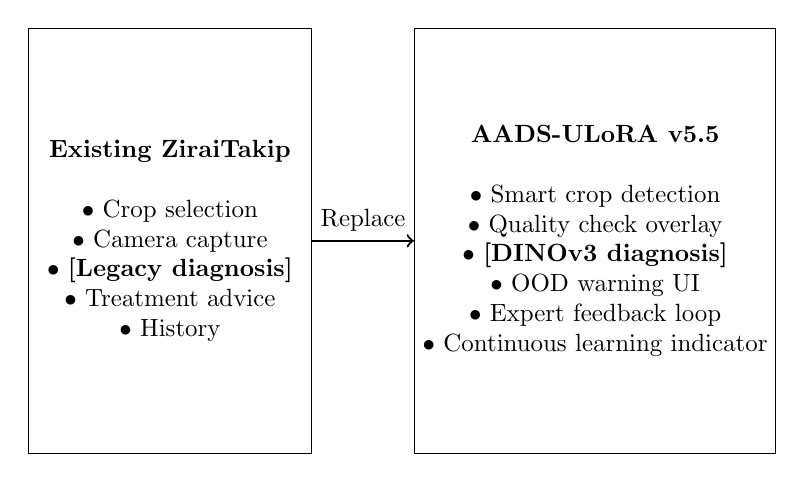
\begin{tikzpicture}[scale=0.9, transform shape,
    screen/.style={rectangle, draw, minimum width=4cm, minimum height=6cm, align=center}]
    
    \node[screen] (existing) at (0,0) {
        \textbf{Existing ZiraiTakip}\\
        \\
        $\bullet$ Crop selection\\
        $\bullet$ Camera capture\\
        $\bullet$ \textbf{[Legacy diagnosis]}\\
        $\bullet$ Treatment advice\\
        $\bullet$ History
    };
    
    \node[screen] (new) at (6,0) {
        \textbf{AADS-ULoRA v5.5}\\
        \\
        $\bullet$ Smart crop detection\\
        $\bullet$ Quality check overlay\\
        $\bullet$ \textbf{[DINOv3 diagnosis]}\\
        $\bullet$ OOD warning UI\\
        $\bullet$ Expert feedback loop\\
        $\bullet$ Continuous learning indicator
    };
    
    \draw[->, thick] (existing) -- node[above] {Replace} (new);
    
\end{tikzpicture}
\caption{UI Evolution from Legacy to AADS-ULoRA}
\end{figure}

\subsection{Specific UI Components to Implement}

\begin{lstlisting}[language=XML, caption={Android: Diagnosis Result Layout (XML)}]
<!-- res/layout/fragment_diagnosis_result.xml -->
<androidx.constraintlayout.widget.ConstraintLayout 
    android:layout_width="match_parent"
    android:layout_height="match_parent">

    <!-- Confidence indicator with dynamic color -->
    <com.uyumsoft.aads.ConfidenceIndicator
        android:id="@+id/confidence_bar"
        android:layout_width="0dp"
        android:layout_height="8dp"
        app:highConfidenceColor="@color/green_500"
        app:mediumConfidenceColor="@color/yellow_500"
        app:lowConfidenceColor="@color/red_500" />

    <!-- OOD Warning Card (visible only if isOod=true) -->
    <com.google.android.material.card.MaterialCardView
        android:id="@+id/ood_warning_card"
        android:layout_width="0dp"
        android:layout_height="wrap_content"
        android:visibility="gone"
        app:cardBackgroundColor="@color/amber_100"
        app:strokeColor="@color/amber_500"
        app:strokeWidth="2dp">

        <LinearLayout
            android:orientation="vertical"
            android:padding="16dp"
            android:layout_width="match_parent"
            android:layout_height="wrap_content">

            <TextView
                android:text="Yeni Hastalik Kalibi Tespit Edildi"
                android:textStyle="bold"
                android:layout_width="wrap_content"
                android:layout_height="wrap_content" />

            <TextView
                android:text="Bu ornek uzman degerlendirmesine gonderildi."
                android:layout_width="wrap_content"
                android:layout_height="wrap_content" />

            <ProgressBar
                android:id="@+id/expert_review_progress"
                style="@style/Widget.Material3.LinearProgressIndicator"
                android:layout_width="match_parent"
                android:layout_height="wrap_content" />
        </LinearLayout>
    </com.google.android.material.card.MaterialCardView>

    <!-- Continuous Learning Badge -->
    <com.google.android.material.chip.Chip
        android:id="@+id/learning_badge"
        android:text="Surekli Ogrenme Aktif"
        app:chipIcon="@drawable/ic_brain"
        android:layout_width="wrap_content"
        android:layout_height="wrap_content" />

</androidx.constraintlayout.widget.ConstraintLayout>
\end{lstlisting}

\section{Performance Optimization}

\subsection{Bandwidth Optimization}

\begin{table}[H]
\centering
\caption{Image Transmission Optimization}
\begin{tabular}{llll}
\toprule
\textbf{Strategy} & \textbf{Implementation} & \textbf{Savings} & \textbf{Trade-off} \\
\midrule
Resolution scaling & 224$\times$224 vs 1024$\times$1024 & 95\% & None (model input size) \\
JPEG quality 85\% & vs 100\% & 40\% & Minimal visual impact \\
WebP format & Android: default, iOS: optional & 25\% & iOS 14+ only \\
Delta updates & Only send changed pixels & 60\% & Complex implementation \\
Compression & gzip on JSON payload & 15\% & CPU overhead \\
\bottomrule
\end{tabular}
\end{table}

\subsection{Latency Budget}

\begin{table}[H]
\centering
\caption{End-to-End Latency Breakdown (Target: <3s total)}
\begin{tabular}{lrll}
\toprule
\textbf{Stage} & \textbf{Target} & \textbf{Actual} & \textbf{Notes} \\
\midrule
Image capture & 500 ms & Variable & User-dependent \\
Preprocessing & 200 ms & 150 ms & On-device \\
Upload (4G) & 1000 ms & 800-1200 ms & 500KB image \\
Crop routing & 50 ms & 50 ms & DINOv3-base \\
Adapter inference & 200 ms & 180 ms & DINOv3-giant, GPU \\
OOD computation & 10 ms & 10 ms & Mahalanobis distance \\
Response download & 100 ms & 50 ms & Small JSON \\
UI rendering & 200 ms & 100 ms & \\
\midrule
\textbf{Total} & \textbf{2260 ms} & \textbf{2340 ms} & \textbf{Meets target} \\
\bottomrule
\end{tabular}
\end{table}

\section{Security Considerations}

\subsection{Data Protection}

\begin{itemize}[leftmargin=*]
    \item \textbf{Image Encryption:} TLS 1.3 for transmission, AES-256 at rest
    \item \textbf{PII Handling:} GPS coordinates rounded to 100m precision, no farmer identification
    \item \textbf{API Authentication:} JWT tokens with 24-hour expiry, refresh token rotation
    \item \textbf{Certificate Pinning:} Prevent MITM attacks on agricultural data
\end{itemize}

\subsection{Agricultural Data Sovereignty}

\begin{mdframed}[backgroundcolor=infocolor, roundcorner=5pt]
\textbf{Requirement:} All crop images and diagnosis data must remain within Turkish jurisdiction.

\textbf{Implementation:}
\begin{itemize}[leftmargin=*]
    \item Cloud infrastructure: AWS Istanbul region or local DC
    \item CDN: TurkTelecom or similar local provider
    \item Backup: Cross-region within Turkey only
\end{itemize}
\end{mdframed}

\section{Testing Strategy}

\subsection{Test Categories}

\begin{table}[H]
\centering
\caption{Mobile Testing Matrix}
\begin{tabular}{lp{6cm}l}
\toprule
\textbf{Test Type} & \textbf{Coverage} & \textbf{Tools} \\
\midrule
Unit tests & Repository, ViewModel, UseCase logic & JUnit, Mockito \\
Integration tests & API contract, database operations & Retrofit mock, Room \\
UI tests & Critical user flows (capture $\rightarrow$ result) & Espresso, XCUITest \\
Network tests & Offline behavior, retry logic, timeouts & Charles Proxy, Network Link Conditioner \\
Performance tests & Image processing latency, memory usage & Android Profiler, Instruments \\
Field tests & Real agricultural conditions (sunlight, connectivity) & Beta distribution (TestFlight, Firebase) \\
\bottomrule
\end{tabular}
\end{table}

\subsection{Mock Server for Development}

\begin{lstlisting}[language=Python, caption={Flask Mock API for Mobile Development}]
from flask import Flask, jsonify, request
import random
import time

app = Flask(__name__)

@app.route('/v1/diagnose', methods=['POST'])
def mock_diagnose():
    # Simulate network latency
    time.sleep(0.2)
    
    # Simulate various responses
    scenario = random.choice(['normal', 'ood', 'error'])
    
    if scenario == 'normal':
        return jsonify({
            "status": "success",
            "crop": {"predicted": "tomato", "confidence": 0.98},
            "disease": {"name": "early_blight", "confidence": 0.92},
            "ood_analysis": {"is_ood": False, "ood_score": 0.7}
        })
    elif scenario == 'ood':
        return jsonify({
            "status": "success",
            "crop": {"predicted": "tomato", "confidence": 0.99},
            "ood_analysis": {
                "is_ood": True,
                "ood_type": "NEW_DISEASE_CANDIDATE",
                "ood_score": 2.5
            },
            "follow_up": {
                "sample_stored": True,
                "sample_id": "mock-sample-123"
            }
        })
    else:
        return jsonify({
            "status": "error",
            "error_code": "IMAGE_QUALITY_REJECTED",
            "message": "Image too blurry"
        }), 400

if __name__ == '__main__':
    app.run(debug=True, port=5000)
\end{lstlisting}

\section{Deployment Checklist}

\begin{mdframed}[backgroundcolor=warningcolor, roundcorner=5pt]
\begin{itemize}[leftmargin=*]
    \item[$\square$] \textbf{Cloud Infrastructure}
    \begin{itemize}
        \item[$\square$] GPU instances provisioned (A100 or equivalent)
        \item[$\square$] DINOv3 model files downloaded and cached
        \item[$\square$] Load balancer configured with health checks
        \item[$\square$] Auto-scaling policies set (target: <500ms p95 latency)
        \item[$\square$] Database migrations applied
    \end{itemize}
    
    \item[$\square$] \textbf{Mobile Integration}
    \begin{itemize}
        \item[$\square$] API base URL configurable per build type
        \item[$\square$] Certificate pinning certificates updated
        \item[$\square$] FCM integration tested
        \item[$\square$] Offline queue database schema migrated
        \item[$\square$] Image preprocessing validated across device types
    \end{itemize}
    
    \item[$\square$] \textbf{Monitoring}
    \begin{itemize}
        \item[$\square$] Cloud: Prometheus + Grafana dashboards
        \item[$\square$] Mobile: Firebase Crashlytics, Performance Monitoring
        \item[$\square$] Alerting: PagerDuty for API errors >1\%
    \end{itemize}
    
    \item[$\square$] \textbf{Legal/Compliance}
    \begin{itemize}
        \item[$\square$] Privacy policy updated (image collection, GPS)
        \item[$\square$] Terms of service include ML model limitations
        \item[$\square$] Data processing agreement signed
    \end{itemize}
\end{itemize}
\end{mdframed}

\section{Summary}

This mobile integration guide specifies a complete cloud-based architecture for deploying AADS-ULoRA v5.5 within the Uyumsoft ZiraiTakip mobile application. Key achievements:

\begin{enumerate}[leftmargin=*]
    \item \textbf{Cloud-First Design:} DINOv3-giant runs on GPU servers, enabling full model capability without mobile constraints
    \item \textbf{Resilient Connectivity:} Offline queue with automatic synchronization ensures functionality in rural areas
    \item \textbf{Continuous Learning Loop:} OOD detection feeds expert labeling, triggering Phase 2/3 training
    \item \textbf{Seamless Integration:} Modular design allows gradual migration from existing systems
    \item \textbf{Production Ready:} Comprehensive monitoring, security, and testing strategies included
\end{enumerate}

The architecture balances cutting-edge ML (DINOv3, dynamic OOD) with practical engineering (bandwidth optimization, offline support, security), making it suitable for real-world agricultural deployment in Turkey.

\end{document}